\begin{abstract}

This is meant as documentation to describe the coordinate system and
units used in \hisparc data and analysis. We also have to deal with
other coordinate systems such as the one used in \corsika and some used
as intermediary in coordinate transformations. The conversions and
relations between these systems are given.

\end{abstract}


\section{Introduction}

Since we have to works with many coordinate systems it can be hard to
keep track of the definitions of each. This document is meant as a
reference to easily find the relations between the different systems.
First coordinate systems used by \hisparc will be discussed. Including
the units that are used and where it is used. Then other coordinate
systems that we have to deal with are discussed, including ways to
convert from those to our usual coordinate systems.


\section{Geographic}

Geographic coordinate systems define a point on the Earth. Multiple
systems are important; WGS84, ECEF and ENU. Additionally a compass based
system is used for detector locations relative to \gps antenna. These
systems are described in the following sections.
\figref{fig:wgs84_ecef_enu} shows the relationships between the global
systems. The conversion formulae are taken from \cite{wikipedia:2014aa}.

\begin{figure}
    \centering
    \tdplotsetmaincoords{70}{95}

\pgfmathsetmacro{\rvec}{.8}
\pgfmathsetmacro{\latitude}{90-45}  % phi
\pgfmathsetmacro{\longitude}{50}  % lambda

\begin{tikzpicture}[scale=5,thick,tdplot_main_coords]

    \definecolor{base}{RGB}{128,128,128}; % grey
    \definecolor{wgs84}{RGB}{255,153,0}; % orange
    \definecolor{ecef}{RGB}{13,98,153}; % blue
    \definecolor{enu}{RGB}{0,184,0}; % green

    \coordinate (O) at (0,0,0);

    % base
    \draw[base] (O) circle (\rvec);
    \draw[base] (\rvec,-.2,0) node[anchor=north east,rotate=-10] {Equator};
    \tdplotsetthetaplanecoords{90};
    \draw[base,tdplot_rotated_coords] (O) circle (\rvec);
    \tdplotsetthetaplanecoords{0};
    \draw[base,tdplot_rotated_coords] (\rvec,0,0) arc (0:90:\rvec)
        node[above right,rotate=88] {Prime Meridian};
    \tdplotsetthetaplanecoords{\longitude};
    \draw[base,dashed,tdplot_rotated_coords] (\rvec,0,0) arc (0:90:\rvec);

    % ECEF
    \draw[ecef,->,-stealth] (O) -- (1,0,0) node[anchor=north]{$X$};
    \draw[ecef,->,-stealth] (O) -- (0,1,0) node[anchor=west]{$Y$};
    \draw[ecef,->,-stealth] (O) -- (0,0,1) node[anchor=south]{$Z$};
    \tdplotsetcoord{P}{\rvec}{\latitude}{\longitude};
    \draw[->,-stealth] (O) -- (P);
    \draw[dashed] (O) -- (Pxy);
    \draw[dashed] (P) -- (Pxy);

    % WGS84
    \tdplotdrawarc[wgs84,->,-stealth]
        {(O)}{0.25}{0}{\longitude}{anchor=north}{$\lambda$};
    \tdplotsetthetaplanecoords{\longitude};
    \tdplotdrawarc[wgs84,->,-stealth,tdplot_rotated_coords]
        {(0,0,0)}{0.25}{90}{\latitude}{anchor=south west}{$\phi$};

    % ENU
    \tdplotsetrotatedcoords{\longitude}{\latitude}{0};
    \tdplotsetrotatedcoordsorigin{(P)};

%   This should be the ENU axes, but I cant find the correct rotation:
%    \draw[enu,tdplot_rotated_coords,->] (0,0,0) -- (.3,0,0) node[anchor=west]{$East$};
%    \draw[enu,tdplot_rotated_coords,->] (0,0,0) -- (0,.3,0) node[anchor=south]{$North$};
%    \draw[enu,tdplot_rotated_coords,->] (0,0,0) -- (0,0,.4) node[anchor=south]{$Up$};

    \draw[enu,->,-stealth,tdplot_rotated_coords] (0,0,0) -- (-.45,0,0)
        node[anchor=south]{$North$};
    \draw[enu,->,-stealth,tdplot_rotated_coords] (0,0,0) -- (0,.45,0)
        node[anchor=west]{$East$};
    \draw[enu,->,-stealth,tdplot_rotated_coords] (0,0,0) -- (0,0,.45)
        node[anchor=south]{$Up$};

\end{tikzpicture}

    \caption{Relationship between the WGS84 (orange), ECEF (blue) and ENU
             (green) coordinate systems.}
    \label{fig:wgs84_ecef_enu}
\end{figure}


\subsection{World Geodetic System 1984 (WGS84)}

For the location of a station we use a \gps antenna. The \gps returns
coordinates in the WGS84 coordinate system. This defines a position with
a latitude, longitude and altitude. The latitude ($\phi$) and longitude
($\lambda$) are defined in decimal degrees, the altitude in meters.
Latitude is the angular distance between a location and the equator,
angles towards north are positive. The longitude is the angular distance
of a location to the Prime Meridian, angles towards east are positive.
The altitude is the height above an ellipsoid that approximates the
shape of the Earth, the parameters that define this ellipsoid are given
in \eqref{eq:wgs84}.


\subsection{Earth-Centered, Earth-Fixed (ECEF)}

This coordinate has its origin as the center of the Earth
(Earth-Centered), and its axes are aligned with the WGS84 system. The
z-axis points to North. The x-axis crosses the Earth where the equator
(\SI{0}{\degree} latitude) intersects with the prime meridan
(\SI{0}{\degree} longitude).

The formulae to convert WGS84 to ECEF are:

\begin{equation}
    \begin{array}{l}
        X = (N + \mathrm{altitude}) \cos{\phi} \cos{\lambda} \ , \\
        Y = (N + \mathrm{altitude}) \cos{\phi} \sin{\lambda} \ , \\
        Z = (\frac{b^2}{a^2} N + \mathrm{altitude}) \sin{\phi} \ . \\
    \end{array}
\end{equation}

Where the ellipsoid is defined by

\begin{equation}
    \label{eq:wgs84}
    \begin{array}{l}
        a = \SI{6378137.0}{\meter} \ , \\
        f = \frac{1}{298.257223563} \ , \\
        b = a (1 - f) \ , \\
        e = \sqrt{2 f - f^2} \ , \\
        N = \frac{a}{\sqrt{1 - e^2 \sin{\phi}^2}} \ , \\
    \end{array}
\end{equation}

\noindent
here $a$ is the semi-major axis, $f$ the flattening, $b$ the semi-minor
axis and $e$ the eccentricity of the ellipsoid. $N$ is the Normal, which
is the distance from the surface of the ellipsoid to the intersection
between the normal of the location on the ellipsoid and the z-axis.


\subsection{East, North, Up (ENU)}

East, North, Up is used by us to easily get distances, relative locations
and angles between locations. It is a local coordinate system where its
origin (reference position) can be chosen. From the reference location
east is the positive x-axis, north is the positive y-axis and up (towards
Zenith) is the positive z-axis. All distances are in meters.

The formulae to convert ECEF to ENU with a reference position are:

\begin{equation}
    \begin{bmatrix}
    x \\ y \\ z
    \end{bmatrix}
    = 
    \begin{bmatrix}
                 -\sin(\lambda_r) &               \cos(\lambda_r) &           0. \\
    -\sin(\phi_r) \cos(\lambda_r) & -\sin(\phi_r) \sin(\lambda_r) & \cos(\phi_r) \\
     \cos(\phi_r) \cos(\lambda_r) &  \cos(\phi_r) \sin(\lambda_r) & \sin(\phi_r)
    \end{bmatrix}
    \begin{bmatrix}
    X - X_r \\ Y - Y_r \\ Z - Z_r
    \end{bmatrix}
\end{equation}

where  $(X, Y, Z)$ and $(x, y, z)$ are the location in ECEF and ENU
respectively. $(\phi_r, \lambda_r)$ and $(X_r, Y_r, Z_r)$ are the
reference position in WGS84 and ECEF respectively.


\subsection{Compass}

For reconstructions of events the location of the individual detectors
are required. To measure the location of detectors in a station we need
to define the positions of detectors relative to the \gps antenna,
because that position is known. We use a simple system that requires a
distance and angle measurement, see \figref{fig:enu_compass}. The
distance (r) between the \gps and a detector (center of the
scintillator) is measured (in meters) the angle ($\alpha$) relative to
the North Pole is determined using a compass. This angle is in degrees
and goes from North to East (NESW). Note that there is a difference
between the magnetic and geographic north pole. The difference can be up
to \SI{3}{\degree} for some \hisparc station locations
\cite{canada:2013aa}. The rotation angle of the detector itself
($\beta$) is defined and the angle of the long side of the detector
relative to the North Pole (positive towards East).

\begin{figure}
    \centering
    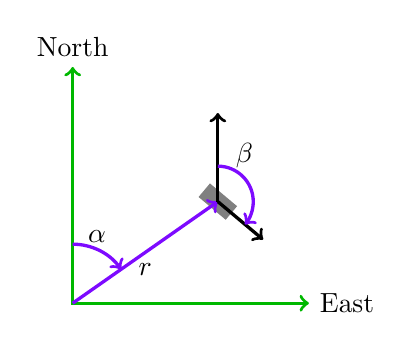
\begin{tikzpicture}[scale=1.5,line width=1.2pt]

  \definecolor{enu}{RGB}{0,184,0} % green
  \definecolor{compass}{RGB}{125,10,255} % purple
  \definecolor{base}{RGB}{128,128,128} % grey

  % Origin
  \coordinate (o) at (0,0);

  % Draw ENU axes
  \draw [enu,<->]
      (0,2) node[black] (yaxis) [above] {North} |-
      (2,0) node[black] (xaxis) [right] {East};

  % Draw a detectors
  \coordinate (d0) at (35:1.5);
  \fill[base,rotate=-40] (d0) ++(-.15,-.075) rectangle +(.3,.15);

  % Draw distance line
  \draw[compass,->] (o) -- node[black,below] {$r$} (d0);
  % Draw angle line
  \draw[compass,->] (0,.5) arc (90:35:.5);
  \draw[compass] (70:.6) node[black] {$\alpha$};

  % Draw North from detector
  \draw[->] (d0) -- +(0,.75);
  % Draw detector angle
  \draw[->] (d0) -- +(-40:.5);

  % Draw angle line
  \draw[compass,->] (d0) ++(0,.3) arc (90:-40:.3);
  \draw[compass] (d0) ++(60:.45) node[black] {$\beta$};

\end{tikzpicture}

    \caption{Relationship between the ENU (green) and Compass (purple)
             coordinate system and how it is used to define the position
             and rotation of a detector.}
    \label{fig:enu_compass}
\end{figure}

The formulae to convert the location of a station in Compass coordinates
to ENU are:

\begin{equation}
    \begin{array}{l}
        x = r * \sin{\alpha} \ , \\
        y = r * \cos{\alpha} \ , \\
        z = z \ . \\
    \end{array}
\end{equation}


\section{Time}

For \hisparc detection events it is important to know precisely when
they occur, a \gps is used to get synchronized and precise timing. This
gives us a timestamp, but this needs to be converted to other time
systems.


\subsection{\gps time}

From they \gps we get a timestamp which are the number of nanoseconds
since the UNIX epoch 1 January 1970 00:00:00.000000000. The \gps
timestamp is a continuously increasing number. This is different from
the UTC timestamp in which certain seconds are repeated when `leap
seconds' are added. Leap seconds are used to keep UTC close to the mean
solar time. Currently the difference between UTC and \gps time is 16
seconds \cite{usno:2012aa}.


\subsection{UTC time}

Similar to \gps but corrected to keep it more in sync with solar time.


\subsection{Julian Date (JD)}

Decimal number to count the number of days since 1 January 4713 B.C.
12:00:00.

Modified Julian Date to keep number shorter uses epoch 17 November 1858
00:00:00. The difference between a Modified Julian Date and a Julian
Date is 2400000.5 days.

\begin{equation}
    MJD = JD - 2400000.5
\end{equation}


\subsection{Greenwich Mean Sidereal Time (GMST)}

Rotation of the prime meridian relative to the vernal equinox, usually
expressed in hours. In a solar day the Earth rotates more than
\SI{360}{\degree} around its axis because it is also in orbit around the
Sun, causing the position of the Sun relative to the Earth to change.
The Earth orbits the Sun every 365.25 days, one day is therefore
approximately \SI{1}{\degree}. So an extra rotation of approximately
\SI{1}{\degree} around its axis is required to get the same part of the
Earth to face the Sun. In sidereal time the rotation of Earth relative
to the `fixed' background stars is taken. A sidereal day is a full
rotation of Earth around its axis. This means around 4 minutes shorter
than a solar day, which needs to rotate a bit further. In
\figref{fig:sidereal_time} the difference between a solar and sidereal
day is illustrated.

\cite{kaplan:2011aa}

\begin{figure}
    \centering
    \pgfmathsetmacro{\rsun}{.2}
\pgfmathsetmacro{\rearth}{.15}
\pgfmathsetmacro{\AU}{1.1}
\pgfmathsetmacro{\margin}{.05}

\pgfmathsetmacro{\orbit}{270}
\pgfmathsetmacro{\siderealday}{32}
\pgfmathsetmacro{\solarday}{50}
\pgfmathsetmacro{\omargin}{10}

\begin{tikzpicture}[scale=2,thick]

    \definecolor{base}{RGB}{128,128,128}; % grey
    \definecolor{sidereal}{RGB}{44,92,198}; % blue
    \definecolor{solar}{RGB}{202,112,27}; % orange
    \definecolor{earth}{RGB}{0,184,0}; % green

    % coordinates
    \coordinate (O) at (0,0);
    \coordinate (earth_0) at (\orbit:\AU);
    \coordinate (earth_1) at (\orbit+\siderealday:\AU);
    \coordinate (earth_2) at (\orbit+\solarday:\AU);

    % Earth
    \draw[base,dashed] (O) circle (\AU);
    \draw[earth] (250:\AU) node[anchor=north east] {Earth};
    \draw[earth,fill=green] (earth_0) circle (\rearth);
    \draw[earth,fill=green] (earth_1) circle (\rearth);
    \draw[earth,fill=green] (earth_2) circle (\rearth);

    % AU
    \draw[base,dashed] (O) -- (earth_0);
    \draw[base,dashed] (O) -- (earth_1);
    \draw[base,dashed] (O) -- (earth_2);

    % Sun
    \draw[solar,fill=yellow] (O) circle (\rsun);
    \draw[solar] (180:\rsun) node[anchor=north east] {Sun};

    % Prime Meridian
    \draw (earth_0) -- ($ (earth_0)!\rearth!(O) $);
    \draw (earth_1) -- ++(90:\rearth);
    \draw (earth_2) -- ($ (earth_2)!\rearth!(O) $);

    % Earth orbit
    \tdplotdrawarc[base,-stealth]
        {(O)}{\AU-\margin}{\orbit+\omargin}{\orbit+\siderealday-\omargin}
        {}{};
    \tdplotdrawarc[sidereal,-stealth]
        {(O)}{\AU+\rearth+\margin+\margin}{\orbit}{\orbit+\siderealday}
        {anchor=north}{Sidereal day};
    \tdplotdrawarc[solar,-stealth]
        {(O)}{\AU+\rearth+\margin}{\orbit}{\orbit+\solarday}
        {anchor=north west}{Solar day};

    % Earth rotation
    \tdplotdrawarc[base,-stealth]
        {(earth_0)}{\rearth-\margin}{110}{430}{anchor=west}{};

    % Earth rotation
    \tdplotdrawarc[base] {(O)}{\rsun+\margin}{\orbit}{\orbit+\siderealday}{}{};
    \tdplotdrawarc[base] {(earth_1)}{\rearth+\margin}{90}{90+\siderealday}{}{};


    % Stellar background
    \draw[sidereal,->] ($ (O) + (90:\rsun+\margin) $) -- ++(90:.2)
        node[anchor=south] {Background stars};
    \draw[sidereal,->] ($ (earth_0) + (90:\rearth+\margin) $) -- ++(90:.2);
    \draw[sidereal,->] ($ (earth_1) + (90:\rearth+\margin) $) -- ++(90:.2);
    \draw[sidereal,->] ($ (earth_2) + (90:\rearth+\margin) $) -- ++(90:.2);

\end{tikzpicture}

    \caption{This shows the orbit of Earth (green) around the Sun
             (yellow). The black line on the Earth represents the prime
             meridian. A full rotation of the Earth causes the prime
             meridian to point to the same background stars, this is a
             sidereal day. It takes longer, due to the orbit of the
             Earth, for the prime meridian to point to the Sun again,
             which is a solar day.}
    \label{fig:sidereal_time}
\end{figure}


\subsection{Local Sidereal Time (LST)}

Similar to GMST but takes observers longitude into account.

To get the Local Sidereal Time the extra angle of the observers
longitude has to be added to the GMST.

\begin{equation}
    \begin{array}{l}
        \mathit{LST} = \mathit{GMST} + \lambda 15 \ . \\
    \end{array}
\end{equation}

\section{Celestial}

Here we describe the different coordinate systems that are used to
define the direction (origin) of an air shower.

\begin{figure}
    \centering
    \tdplotsetmaincoords{70}{95}

\pgfmathsetmacro{\rlen}{1.8}
\pgfmathsetmacro{\latitude}{90-45}  % phi
\pgfmathsetmacro{\longitude}{120}  % lambda

\pgfmathsetmacro{\clen}{3}
\pgfmathsetmacro{\ra}{33}  % right ascension in degrees
\pgfmathsetmacro{\dec}{90-50}  % declination in degrees

\pgfmathsetmacro{\gmst}{-45}  % Greenwich mean sidereal time
\pgfmathsetmacro{\lst}{\longitude+\gmst}  % local sidereal time in degrees

%\pgfmathsetmacro{\zenith}{22}  % theta
%\pgfmathsetmacro{\azimuth}{0}  % phi

\begin{tikzpicture}[scale=2,thick,tdplot_main_coords]

    \definecolor{base}{RGB}{128,128,128}; % grey
    \definecolor{wgs84}{RGB}{255,153,0}; % orange
    \definecolor{ecef}{RGB}{13,98,153}; % blue
    \definecolor{enu}{RGB}{0,184,0}; % green
    \definecolor{compass}{RGB}{125,10,255}; % purple
    \definecolor{equa}{RGB}{253,39,39}; % red
    \definecolor{time}{RGB}{15,171,135}; % teal

    \coordinate (O) at (0,0,0);

    % base
    \draw[base] (O) circle (\rlen);
    \draw[base] (\rlen,-.2,0);  % Equator
    \tdplotsetthetaplanecoords{90};
    \draw[base,tdplot_rotated_coords] (O) circle (\rlen);
    \tdplotsetthetaplanecoords{\gmst};
    % Prime Meridian
    \draw[base,tdplot_rotated_coords] (\rlen,0,0) arc (0:90:\rlen);
    \tdplotsetthetaplanecoords{\lst};
    \draw[base,dashed,tdplot_rotated_coords] (\rlen,0,0) arc (0:90:\rlen);
    \draw[base,dashed,tdplot_rotated_coords] (\clen,0,0) arc (0:90:\clen);
    \draw[base,dashed,tdplot_rotated_coords] (0,0,0) -- (0,\clen,0);

    % celestial base
    \draw[base] (O) circle (\clen);
    \draw[base] (\clen,-.8,0)
        node[anchor=north east,rotate=-10] {Celestial Equator};
    \draw[base,->,-stealth] (O) -- (0,0,\clen + .3)
        node[anchor=south] {Celestial North Pole};
    \tdplotsetthetaplanecoords{90};
    \draw[base,tdplot_rotated_coords] (O) circle (\clen);

    % ECEF
    \tdplotsetrotatedcoords{0}{0}{\gmst};
    \draw[ecef,->,-stealth,tdplot_rotated_coords] (O) -- (\rlen+.2,0,0)
        node[anchor=north] {$X$};
    \draw[ecef,->,-stealth,tdplot_rotated_coords] (O) -- (0,\rlen+.2,0)
        node[anchor=west] {$Y$};
    \draw[ecef,->,-stealth,tdplot_rotated_coords] (O) -- (0,0,\rlen+.2)
        node[anchor=west] {$Z$};

    % WGS84
    % longitude
    \tdplotsetrotatedcoords{0}{0}{\gmst};
    \tdplotdrawarc[wgs84,->,-stealth,tdplot_rotated_coords]
        {(O)}{0.4}{0}{\longitude}{anchor=north}{$\lambda$};
    % latitude
    \tdplotsetthetaplanecoords{\lst};
    \tdplotdrawarc[wgs84,->,-stealth,tdplot_rotated_coords]
        {(0,0,0)}{0.4}{90}{\latitude}{anchor=west}{$\phi$};

    % gmst
    \tdplotsetthetaplanecoords{\lst};
    \tdplotdrawarc[time,->,-stealth]
        {(O)}{\rlen}{0}{360+\gmst}{anchor=south}{GMST};
    \tdplotdrawarc[time,->,-stealth]
        {(O)}{\clen}{\lst}{\ra}{anchor=north west}{HA};

    % observer
    \tdplotsetcoord{P}{\rlen}{\latitude}{\lst};
    \tdplotsetcoord{P'}{\clen}{\latitude}{\lst};
    \draw[color=black,->,-stealth] (O) -- (P);
    \draw[base] (P) -- (P') node[anchor=south west] {Zenith};
    \draw[base,dashed] (P) -- (Pxy);

    % Equatorial
    \draw[base,->,-stealth] (O) -- (\clen + .3,0,0)
        node[anchor=north]{$\vernal$};

    \tdplotsetcoord{S}{\clen}{\dec}{\ra};
    \draw[->,-stealth] (O) -- (S) node[anchor=south west] {$\star$};
    \draw[base,dashed] (S) -- (Sxy);

    \tdplotsetthetaplanecoords{\ra};
    \draw[base,dashed,tdplot_rotated_coords] (\clen,0,0) arc (0:90:\clen);
    \draw[base,dashed,tdplot_rotated_coords] (0,0,0) -- (0,\clen,0);
    \tdplotdrawarc[equa,->,-stealth,tdplot_rotated_coords]
        {(0,0,0)}{\clen}{90}{\dec}{anchor=west}{$\delta$};
    \tdplotdrawarc[equa,->,-stealth]
        {(O)}{\clen}{0}{\ra}{anchor=north}{$\alpha$};

\end{tikzpicture}

    \caption{Relationship between the WGS84 (orange), ECEF (blue),
             Equatorial (red) and clock (teal) coordinate systems.
             $\vernal$ points to the vernal equinox, the point where the
             ecliptic and celestial equator cross in the Aries zodiac.}
    \label{fig:wgs84_equatorial}
\end{figure}


\subsection{Zenith and Azimuth}

When a station detects a shower we try to reconstruct the direction of
its origin. The direction of a shower is then given by an zenith and
azimuth coordinate. These coordinates define a point on the semi-sphere
that is the sky above the detection station. The Zenith is the point
directly above the observer. The zenith angle is the angle between the
direction and the Zenith point. The azimuth is the direction in the
horizontal plane, it starts at East (\SI{0}{\radian}) then goes to North
(ENWS).

We do not expect nor consider air showers from below the horizon, so the
zenith angles, defined in radians, are an angle in the range [0,
$\frac{\pi}{2}$). The azimuth is restricted to the range [$-\pi$, $\pi$).

\begin{figure}
    \centering
    \tdplotsetmaincoords{70}{-10}

\pgfmathsetmacro{\rlen}{.8}
\pgfmathsetmacro{\zenith}{90-45}  % theta
\pgfmathsetmacro{\azimuth}{300}  % phi

\begin{tikzpicture}[scale=5,thick,tdplot_main_coords]

    \definecolor{base}{RGB}{128,128,128}; % grey
    \definecolor{wgs84}{RGB}{255,153,0}; % orange
    \definecolor{ecef}{RGB}{13,98,153}; % blue
    \definecolor{enu}{RGB}{0,184,0}; % green
    \definecolor{zenazi}{RGB}{200,20,200}; % pink
    \definecolor{hori}{RGB}{200,180,20}; % gold

    % coordinates
    \coordinate (O) at (0,0,0);
    \tdplotsetcoord{P}{\rlen}{\zenith}{\azimuth};

    % base
    \draw[base] (O) circle (\rlen);
    \draw[base] (-\rlen*.8,-\rlen*.8,0) node[anchor=west,rotate=-10] {Horizon};
    \tdplotsetthetaplanecoords{\azimuth};
    \draw[base,dashed,tdplot_rotated_coords] (\rlen,0,0) arc (0:90:\rlen);
    \draw[base,dashed,tdplot_rotated_coords] (0,0,0) -- (0,\rlen,0);
    \draw[base,dashed] (P) -- (Pxy);

    % ENU
    \draw[enu,->,-stealth] (O) -- (1,0,0) node[anchor=west]{East};
    \draw[enu,->,-stealth] (O) -- (0,1,0) node[anchor=south east]{North};

    % Zenith Azimuth
    \tdplotdrawarc[zenazi,->,-stealth]
        {(O)}{0.2}{0}{\azimuth}{anchor=south east}{$\phi$};

    % Horizontal
    \tdplotdrawarc[hori,->,-stealth]
        {(O)}{0.4}{90}{\azimuth-360}{anchor=south west}{$A$};

    \tdplotsetthetaplanecoords{\azimuth};
    % Zenith Azimuth
    \tdplotdrawarc[zenazi,->,-stealth,tdplot_rotated_coords]
        {(0,0,0)}{0.25}{0}{\zenith}{anchor=south west}{$\theta$};
    % Horizontal
    \tdplotdrawarc[hori,->,-stealth,tdplot_rotated_coords]
        {(0,0,0)}{0.25}{90}{\zenith}{anchor=south west}{$a$};

    % ENU
    \draw[enu,->,-stealth] (O) -- (0,0,1) node[anchor=south]{Up};

    % star
    \draw[->,-stealth] (O) -- (P) node[anchor=south west] {$\star$};

\end{tikzpicture}

    \caption{Relationship between the ENU (green), Zenith Azimuth (pink)
             and horizontal (gold) coordinate systems.}
    \label{fig:enu_horizontal}
\end{figure}


\subsection{Horizontal}

This is a system used as intermediary for some coordinate conversions.
It uses azimuth ($A$) and altitude ($a$) to define a direction. The
altitude is the opposite of the zenith, so \SI{0}{\radian} is horizontal
and \SI{\pi / 2}{\radian} is the zenith. The azimuth definition also
differs, in Horizontal coordinates it moves from North to East (NESW).

The formulae to convert from zenith ($\theta$) and azimuth ($\phi$) to
altitude ($a$) and azimuth ($A$) are:

\begin{equation}
    \begin{array}{l}
        a = \frac{\pi}{2} - \theta \ , \\
        A = - (\phi + \frac{\pi}{2}) \ . \\
    \end{array}
\end{equation}


\subsection{Equatorial (J2000)}

Vernal equinox, epoch.
Right ascension, Declination, J2000
In decimal hours.

Given an observers position in WGS84, a time of observation in LST and
horizontal coordinates pointing to the source the following formulae can
be used to get the corresponding equatorial coordinates \cite[p.
37]{duffet-smith:1990aa}.

\begin{equation}
    \begin{array}{l}
        \delta = \arcsin{((\sin{a} \sin{\phi}) +
                          (\cos{a} \cos{\phi} \cos{A}))} \ , \\
        \mathit{HA} = \arccos{(\frac{\sin{a} - (\sin{\phi} \sin{\delta})}
                                    {\cos{\phi} \cos{\delta}})} \ , \\
        \alpha = \mathit{LST} - \mathit{HA} \ . \\
    \end{array}
\end{equation}

Where $\phi$ the geographical latitude, $a$ the altitude, $A$ the
azimuth, $\mathit{LST}$ the Local sidereal time, $\delta$ is the
declination, $\alpha$ the right ascension and the intermediate variable
$\mathit{HA}$ is the hour angle.


\section{\corsika}

\corsika an extensive air shower simulation program which we use.
\corsika uses a coordinate system which is slightly different from the
ENU system that we use \cite{heck:2013aa}.

\begin{figure}
    \centering
    \tdplotsetmaincoords{70}{-10}

\pgfmathsetmacro{\rlen}{.8}
\pgfmathsetmacro{\zenith}{90-45}  % theta
\pgfmathsetmacro{\azimuth}{40}  % phi

\begin{tikzpicture}[scale=5,thick,tdplot_main_coords]

    \definecolor{base}{RGB}{128,128,128}; % grey
    \definecolor{wgs84}{RGB}{255,153,0}; % orange
    \definecolor{ecef}{RGB}{13,98,153}; % blue
    \definecolor{enu}{RGB}{0,184,0}; % green
    \definecolor{hori}{RGB}{200,20,200}; % pink
    \definecolor{corsika}{RGB}{151,115,0}; % brown

    % coordinates
    \coordinate (O) at (0,0,0);
    \tdplotsetcoord{P}{\rlen}{\zenith}{\azimuth};
    \tdplotsetcoord{P'}{\rlen}{180-\zenith}{180 + \azimuth};

    % base
    \draw[base] (O) circle (\rlen);
    \draw[base] (-\rlen*.8,-\rlen*.8,0) node[anchor=west,rotate=-10] {};
    \tdplotsetthetaplanecoords{\azimuth};
    \draw[base,dashed,tdplot_rotated_coords] (\rlen,0,0) arc (0:90:\rlen);
    \draw[base,dashed] (P) -- (Pxy);
    \draw[base,dashed] (P') -- (P'xy);
    \draw[base,dashed,tdplot_rotated_coords] (0,-\rlen,0) -- (0,\rlen,0);

    % Horizontal
    \tdplotdrawarc[hori,-stealth]
        {(O)}{0.3}{0}{\azimuth}{anchor=west}{$\phi$};
    \tdplotsetthetaplanecoords{\azimuth};
    \tdplotdrawarc[hori,-stealth,tdplot_rotated_coords]
        {(0,0,0)}{0.2}{0}{\zenith}{anchor=south}{$\theta$};

    % ENU
    \draw[enu,-stealth] (O) -- (1,0,0) node[anchor=west]{East};
    \draw[enu,-stealth] (O) -- (0,1,0) node[anchor=south east]{North};
    \draw[enu,-stealth] (O) -- (0,0,1) node[anchor=south east]{Up};

    % CORSIKA
    \tdplotdrawarc[corsika,-stealth]
        {(O)}{0.3}{90}{\azimuth+180}{anchor=south}{$\Phi$};
    \tdplotsetthetaplanecoords{\azimuth};
    \tdplotsetrotatedcoordsorigin{(P)};
    \tdplotdrawarc[corsika,-stealth,tdplot_rotated_coords]
        {(0,0,0)}{0.2}{180}{180+\zenith}{anchor=north}{$\Theta$};

    \draw[corsika,->,dashed,-stealth] (O) -- (-1,0,0) node[anchor=east]{$y$};
    \draw[corsika,->,dashed,-stealth] (O) -- (0,1,0) node[anchor=south west]{$x$};
    \draw[corsika,->,dashed,-stealth] (O) -- (0,0,1) node[anchor=south west]{$z$};

    % star
    \draw[-stealth] (O) -- (P) node[anchor=south west] {$\star$};
    \draw[base,-stealth] (O) -- (P');

\end{tikzpicture}

    \caption{Relationship between the ENU (green), horizontal (pink)
             and CORSIKA (brown) coordinates.}
    \label{fig:enu_corsika}
\end{figure}


\subsection{Geographic}

\corsika defines positions on the ground (or observation level) relative
to the point where the shower axis intersects the observation level.
Positive x axis points to magnetic North, positive y axis to the West,
and the z axis upwards.

The formulae to convert CORSIKA to ENU are:

\begin{equation}
    \begin{array}{l}
        x_{\mathrm{ENU}} = -y_{\mathrm{CORSIKA}} \ , \\
        y_{\mathrm{ENU}} = x_{\mathrm{CORSIKA}} \ , \\
        z_{\mathrm{ENU}} = z_{\mathrm{CORSIKA}} \ . \\
    \end{array}
\end{equation}


\subsection{Celestial}

\corsika looks from the point of view of the shower, so not the
direction it came form, but the direction it goes to. The $\Theta$ angle
is defined the same as our definition of zenith ($\theta$),
\SI{0}{\radian} is a shower from the zenith and \SI{\pi / 2}{\radian} is
a horizontal shower. The $\Phi$ angle is defined differently than our
definition of azimuth ($\phi$). First it is the angle the shower is heading
towards. \SI{0}{\radian} is a shower heading towards North, so coming
form South, which we would define as \SI{\pi / 2}{\radian}. The
(positive) rotation of the angle is in the same direction, from North to
West.

The formulae to convert the CORSIKA direction to our azimuth and zenith are:

\begin{equation}
    \begin{array}{l}
        \theta = \Theta \ , \\
        \phi = \Phi - \frac{\pi}{2} \ . \\
    \end{array}
\end{equation}


\printbibliography
